\documentclass[12pt]{article}
\usepackage[utf8]{inputenc}
\usepackage{graphicx}
\usepackage[margin=2cm]{geometry}
\usepackage{titlesec}
\usepackage{titling}
\usepackage{lipsum}
\usepackage{fancyhdr}
\usepackage{rotating}
\usepackage{hyperref}
\usepackage{enumitem}
\usepackage{tikz}
% \usepackage{standalone}
\usepackage{pdfpages}
\usepackage{listings}
\lstset{
  basicstyle=\ttfamily,
  columns=fullflexible,
  frame=single,
  breaklines=true,
}
\graphicspath{{./resources/}}

\newcommand{\bb}[1]{\textbf{\textit{#1}}}
\newcommand{\tco}{Touriscov}

\hypersetup{
    colorlinks=true,
    linkcolor=blue,
    filecolor=magenta,      
    urlcolor=cyan,
    pdftitle={miniMBAProject},
    pdfpagemode=FullScreen,
    }

\lhead{
\includegraphics[scale=0.1]{iskala-logo.png}}
\chead{}
\rhead{}
\lfoot{}
\cfoot{\thepage}
\rfoot{}

\renewcommand{\thefigure}{}

\renewcommand{\maketitle}{
\begin{center}

    \vspace{1em}
    \large February 12\textsuperscript{th}, 2025
\end{center}
}


\title{MBA Assignment}
\author{Amr Wahdan}
\date{Thursday, May 11th 2023}

\begin{document}
\pagenumbering{0}

\begin{center}
   \topskip8cm
    
\includegraphics[width=0.9\textwidth]{iskala-logo.png}
\end{center}
\vspace{1em}
\begin{center}
    \scalebox{2}{\Large\textbf{Cold Outreach Strategy}}
\end{center}
\vspace{1em}
\maketitle
\pagenumbering{roman}
\newpage


\begin{center}
    \Large\bfseries Cold Emailing for Success
    \vspace{0.5em}
    \hrule\vspace{0.2em}\hrule
\end{center}

\vspace{1em}
\begin{itemize}
    \item Cold emailing is a direct and highly effective method of reaching out to potential business clients, introducing your product or service, and sparking meaningful conversations. In the B2B space, cold emailing allows you to engage with decision-makers who may not be actively seeking your solution, but could benefit from what you offer.
    \item To succeed with cold emailing, especially in a competitive B2B environment, you need a well-defined Ideal Customer Profile (ICP). This helps ensure your outreach is targeted and relevant, reaching the right people with the right message. For example, when targeting business leaders in industries like SaaS, Marketing, and Fintech, your cold emails should clearly highlight how your product or service can solve specific pain points relevant to those industries.
    \item One of the key principles of successful cold emailing is to offer something valuable right from the start---a lead magent. Your message should be brief, personalized, and solution-oriented. By focusing on the recipient's needs and demonstrating how your solution can help them overcome challenges or achieve goals, you can capture their attention and prompt action.
    \item Additionally, aligning your outreach with a strategic cadence — meaning the timing and sequence of your emails — is essential. You may need to follow up several times, each time offering new insights or value, while maintaining a balance between persistence and respect for the prospect’s time.
    \item In summary, cold emailing is a powerful tool in B2B lead generation when used correctly. By understanding your audience, crafting a compelling offer, and employing a well-thought-out outreach cadence, you can engage prospects effectively, build trust, and drive meaningful business relationships.
\end{itemize}

\vspace{2em}
\begin{center}
    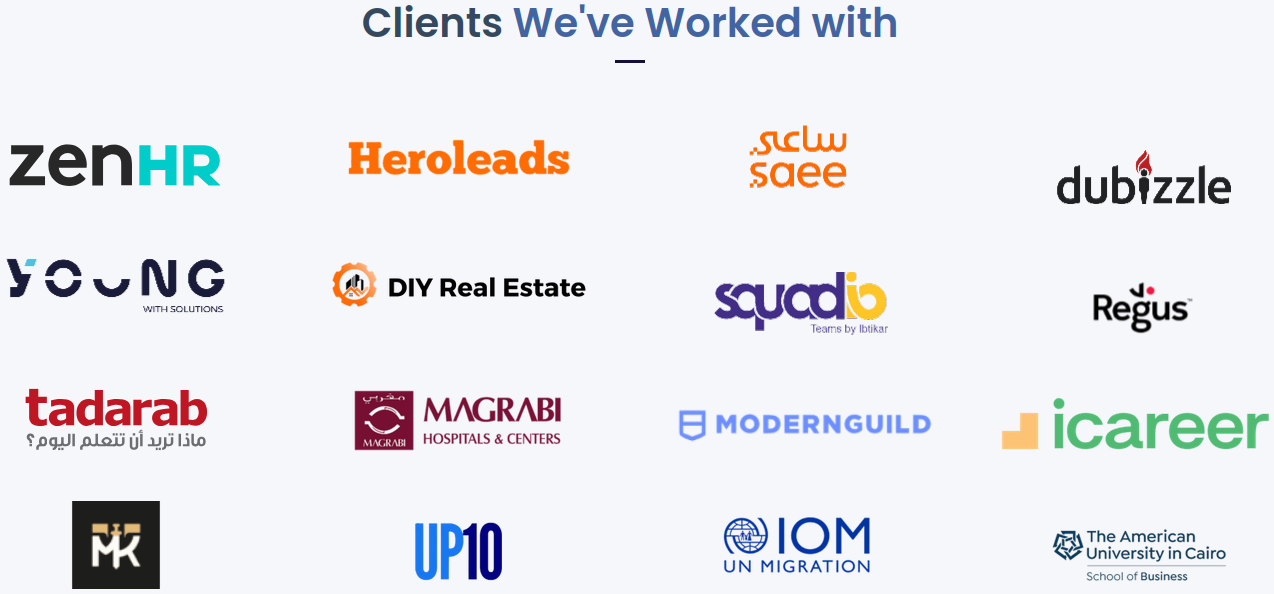
\includegraphics[width=0.8\paperwidth]{iskala-clients.png}  
\end{center}

\newpage
\pagenumbering{arabic}
\pagestyle{fancy}
\topskip2cm
\section{The Cold Part in Cold emailing}
Cold emailing is called "cold" for a reason—it means reaching out to someone who has no prior relationship with you or your business. Unlike warm or hot leads, cold prospects haven’t expressed direct interest in your offer, making your approach crucial in capturing their attention and moving them toward engagement. \par

Since cold emails are unsolicited, they often face skepticism, resistance, or outright dismissal. Many recipients are busy decision-makers who receive countless pitches daily, making it even more challenging to stand out. However, when done correctly, cold emailing can be a powerful tool for opening doors, starting conversations, and generating high-quality leads. \par

\subsection{The Challenges of Cold Outreach}
\begin{enumerate}[label= \roman*.]
	\item \bb{Lack of Awareness:} Since your prospect doesn’t know you, your first challenge is building credibility and trust quickly.
	\item \bb{High Competition:} Many businesses use cold emailing, meaning your email needs to be compelling enough to rise above the noise.
	\item \bb{Spam Filters and Deliverability Issues:} If your emails aren’t properly crafted and optimized, they might never even reach the recipient’s inbox. 
	\item \bb{Low Response Rates:} Since the prospect hasn’t actively sought your solution, conversion rates tend to be lower compared to warm leads.
\end{enumerate}

\subsection{How to cook your emails for leads}
To launch a successful email campaign, you need three things: \textbf{Good data, good emails, and good email sending infrastructure} \par

\section{Data Data Data}
The success of a cold email campaign starts with high-quality data. If you’re reaching the wrong people or using outdated contact information, even the best-crafted email won’t get results. Good data ensures your emails land in the right inboxes, increasing response rates and minimizing wasted effort.\par

\textbf{Why Good Data Matters:}
\begin{itemize}
	\item \bb{Better Deliverability:} Valid emails reduce bounce rates and keep your domain reputation strong.
	\item \bb{Higher Engagement:} Targeting the right decision-makers leads to more responses.
	\item \bb{Efficient Outreach:} Quality data saves time by focusing efforts on prospects who actually fit your Ideal Customer Profile (ICP).
\end{itemize}

\subsection*{How to Get High-Quality Data for Cold Emailing}
\begin{itemize}
	\item \bb{Use Reliable Data Sources:} Platforms like Apollo.io, LinkedIn Sales Navigator, and Crunchbase provide verified B2B contacts.
	\item \bb{Define Your ICP Clearly:} Filter leads by industry, company size, job title, and location to match your ideal prospect profile and actually reach the decision-makers.
	\item \bb{Verify Email Addresses:} Use tools like NeverBounce, ZeroBounce, or Hunter.io to check for valid emails before sending to ensure you're not wasting your time on bad emails.
	\item \bb{Enrich Your Data:} Gather additional details like recent funding, hiring activity, or company news to personalize your outreach. \textbf{CLAY!}
\end{itemize}


\section{Craft an email that converts}
To write an email that delivers, you need to finely tune every aspect of your email to catch your reader's attention, and to have the blessing of the algorithm.

\subsection*{personalization}
\begin{minipage}{.5\textwidth}
	Have you ever gotten one of those Christmas texts that you are 100\% sure were sent to the entire friend group? Do you remember feeling anything after seeing it? I bet not much if any! Emails are no different. Email personalization goes beyond just using a recipient’s name—it’s about making your message relevant to their specific needs, challenges, and interests. In cold emailing, personalization helps break through the noise and makes your email feel less like a mass pitch and more like a tailored solution. \par

\end{minipage}%
\hfill
\begin{minipage}{.5\textwidth}
\begin{flushright}
  \begin{center}
  \vspace{1em}
    
\includegraphics[scale=0.03]{christmas.jpeg}
  \end{center}
  \end{flushright}
\end{minipage}

\vspace{2em}
There are lots of ways to personalize an email---and on many levels too! Here are some of the ways we recommend: \par

\begin{itemize}
	\item \bb{Mentioning Their Company or Industry:} Show you’ve done your research by referencing specific challenges or trends relevant to their field.
	\item \bb{Acknowledge Their Role:} Tailor your message based on their job title and responsibilities.
	\item \bb{Reference Recent Events:} Comment on a company announcement, a LinkedIn post, or an industry trend they’ve been involved in.
\end{itemize}

This will be an ongoing theme in our discussion of cold emails. Every aspect of your email needs to be personalize and tailored to your ICP. \par


\subsection*{Cold Email Anatomy}
Your cold email is broken down into a couple sections: \textbf{Subject line, Intro Line, Offer, and a Call To Action}.

\begin{figure}[h]
	\begin{center}
		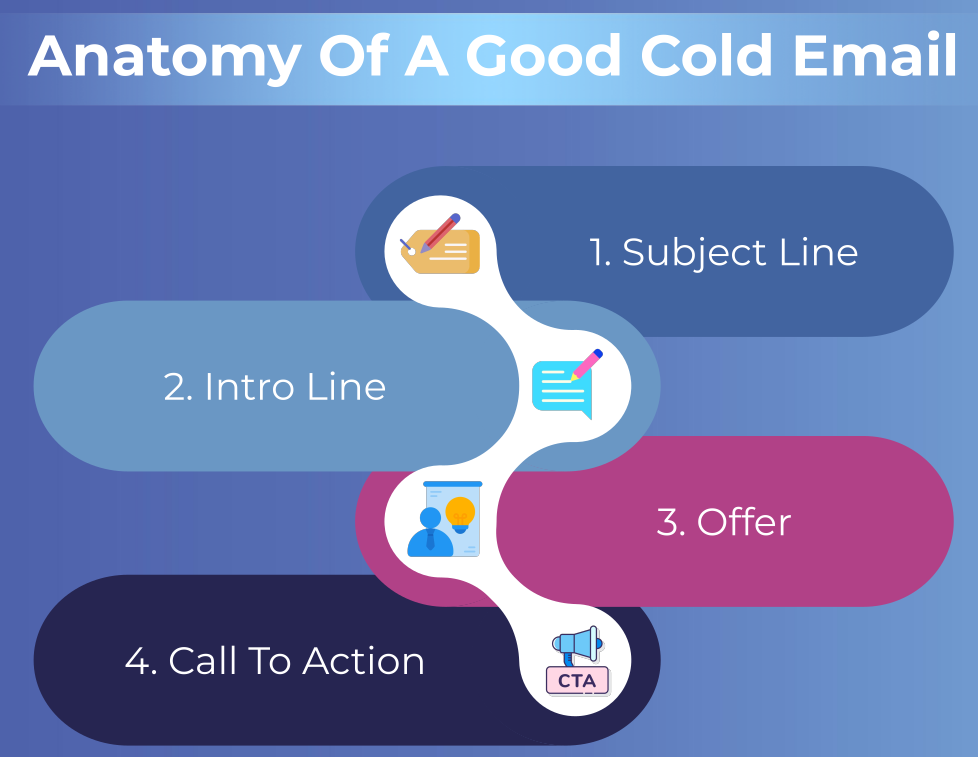
\includegraphics[width=0.7\textwidth]{resources/anatomyemail.png}
	\end{center}
\end{figure}


\subsection{Your subject line}
Your subject line is your frontdoor knocker! You make your first impression by have a solid subject line that breaks the ice, doesn't look or sound spammy, and piques your reader's interest.

You write a good subject line by making it:
\begin{itemize}
	\item \bb{Short, Clear, and Catchy:} Short to actually get read and to appear in full on mobile devices, and clear and catchy to get opened.
	\item \bb{Personalized:} Mention something personal to the reader to grab attention.
	\item \bb{Curiosity-Driven:} Make the reader want to open the email by hinting at something valuable.
	\item \bb{Casual and Conversational:} And I cannot emphasize this enough! You need to sound like you are actually curious, actually striking a conversation, and not just like any other robotic salesperson.
\end{itemize}

\subsection*{Examples of subject lines that work:}
\begin{enumerate}
	\item \{\{First Name\}\}, quick question about \{\{company\}\}
	\item \{\{First Name\}\}, growth meeting?
	\item Partnership: \{\{Your company\}\} <> \{\{Their company\}\}
	\item \{\{First Name\}\}, saw your LinkedIn profile
\end{enumerate}


\subsection{Intro Line}
Your intro line is the first sentence of your email, and it determines whether your prospect keeps reading or moves on. Since cold emails are unsolicited, your opening needs to be engaging, relevant, and \textbf{straight to the point}.\par

I think you got the point---It needs to be personal! It has to be about something specific to your prospect. DO NOT GREET THEM! Instead, compliment a recent promotion they got, an achievement they made, a recent market trend, etc. \par

Good intro lines include:
\begin{itemize}
	\item Noticed your recent post on \{\{topic\}\}, and I had to reach out.
	\item Saw \{\{Company\}\} new brand image. Looks neat!
	\item I saw that \{\{Company\}\} is expanding in \{\{market\}\}—exciting times!
\end{itemize}

\subsection{Compelling Offer}
This is the meat of your cold emailing campaing. Your offer is the most important part of your cold email---it’s what determines whether your prospect takes action or ignores your message. A great offer isn’t just about what you sell; it’s about how your product or service solves a \textbf{specific problem} for the recipient in a way that feels irresistible. \par

If your offer sucks or if your market is really saturated, no copywriting will save you! To craft an offer that sells, we recommend using Alex Hormozi's method that was explained in his book \textit{\$100M Offers}. \par

What makes an offer compelling then?

\begin{itemize}
	\item \bb{Clear Value Proposition:} Your email should immediately answer: Why should they care?
	\item \bb{Specific and Outcome-Focused:} Instead of talking about features, highlight the tangible benefits your prospect will get.
	\item \bb{Low Risk, High Reward:} Reduce hesitation by offering guarantees, free trials, or risk-free consultations.
	\item \bb{Make it short:} Do not go on listing everything you do. Use an elevator pitch instead.
\end{itemize}

And remember to introduce credibility! This is crucial. Provide testimonials, case studies, or good reviews from past projects. Your prospect needs to \textbf{trust} you to be interested in what you have to say/sell.

Revist Hormozi's value equation! This is a simple formula:

\begin{itemize}
	\item \{\{Your Company\}\} helps \{\{Their Company\}\} get \{\{Value Prop\}\} with less \{\{pain point\}\}. Check out \{\{Case Study\}\}.
\end{itemize}

\subsection{Harvest your leads with a CTA}
Your call to action (CTA) is the most important part of your email—it tells the prospect what to do next. A weak or unclear CTA leads to inaction, while a strong one guides the recipient toward a simple, low-friction next step. \par

Not including a strong CTA = losing deals. Your CTA should be simple, easy to find, introduces \textbf{low-friction} next steps for prospects.

Try to introduce a lead magnet here! Offer something free and introduce urgency.

Here are some exmaples for that too:

\begin{itemize}
	\item Would you be interested in \{\{value\}\}? Let me know.
	\item I can offer some insights into how to overcome \{\{pain point\}\}
	\item I can give you \{\{value\}\} for free. Sign up here.
	\item This \{\{value\}\} was made for \{\{company\}\}, would you like to see it before we talk more?
\end{itemize}

\section{Technical infrastructure}

Creative matters aside, marketing is all about \textbf{volume}. You need to get your email to your prospect's inbox, to keep doing it, and to get it in lots of other people's inboxes. \par

To get that done, you need good technical infrastructure. You need to utilize tools to verify emails, A/B test email copies, and to mass send emails. Tools like instantly.ai and smartlead, hunter.io and snov.io, and many many more that will boost your results and help you with your cold emailing campaigns. \par

\begin{minipage}{.5\textwidth}
\begin{flushright}
  \begin{center}
  \vspace{1em}
    
\includegraphics[scale=0.7]{instantly.jpeg}
  \end{center}
  \end{flushright}
\end{minipage}%
\hfill
\begin{minipage}{.5\textwidth}
\begin{flushleft}
  \begin{center}
  \vspace{1em}
    
\includegraphics[scale=0.7]{smartlead.jpeg}
  \end{center}
  \end{flushleft}
\end{minipage}

\newpage 


\section{Strategy for iSkala}
\subsection{Define ICP}
iSkala's ICP includes decision-makers in Marketing, Business Development, Growth or Sales. We can target titles like:
\begin{itemize}
	\item CEO  
    \item Founder  
    \item Co-Founder  
    \item Managing Partner  
    \item Head of Marketing  
    \item Director of Marketing  
    \item Marketing Manager  
    \item Head of Digital Marketing  
    \item Director of Digital Marketing  
    \item Digital Marketing Manager  
    \item Head of Growth  
    \item Director of Growth  
    \item Growth Manager  
    \item Head of Business Development  
    \item Director of Business Development  
    \item Business Development Manager  
    \item Head of Sales  
    \item Director of Sales  
    \item Sales Manager  
\end{itemize}

All of these are people that could read our email and take some sort of action. Most of them having the authority to spend their budget on our product/service.

\subsection{Get Data for ICP}
Utilize services like \url{Apollo.io}, \url{Zoominfo.com}, and others to get very specific and targeted data for your ICP. Make sure to segment your audience and filter the results as much as possible to get best results.

\subsection{Offer Package (Alex Hormozi's \$100M Offers Framework)}
To create an irresistible offer, it should be valuable, desirable, and have a high perceived value with minimal risk. Using Hormozi’s framework, iSkala’s offer should include: \par

\begin{itemize}
	\item We help SaaS business get 50 interested leads per month without breaking the bank.
	\item iSkala works with marketing teams to add 50 high-quality interested leads.
	\item iSkala helps KSA-based companies reach interested prospects in as short as one week.
	\item The iSkala team provides growing UAE startups add 50 guaranteed interested leads per month into their sales funnel.
	\item Our experts at iSkala use tailored copywriting and state of the art tech for email Deliverability to provide its partneres 50 intersted leads per month.
\end{itemize}

\subsection{Credibility}
Include relevant case studies iSkala's team has worked on and the results they got. Check here for more: \url{leadgen.iskala.net/Case-Studies}

\subsection{Performance Monitoring}
Make sure to A/B test the email copies, mointor campaign KPIs, and check the health of the campaign infrastructure.

\newpage 


\section{Example Email Copies}

\begin{lstlisting}
	Subject: Quick question, [First Name]

	Hey [First Name],

	I came across [Company] and noticed you’re scaling in [Industry]. Many 
	[Job Title]s I speak with struggle to consistently book qualified sales meetings without relying on ads or outbound SDRs.

	At iSkala, we help B2B companies like [Competitor] generate [X] booked meetings per month using cold email—without spam or deliverability issues.

	Would it be worth a 10-minute chat this week to see if this could work for you?

	Reply with "NO" if you do not want any further communication.

	Best,
	[Your Name]
\end{lstlisting}

\begin{lstlisting}
	Subject: [First Name], this worked for [Competitor]

	Hey [First Name],

	We recently helped [Competitor] book [X] meetings in [Y] days using cold email—without paid ads or hiring extra sales reps.

	If [Competitor] is seeing success with this, I thought [Company] might benefit too.

	Would love to share how we’re helping [industry] companies scale their pipeline. I can send a quick demo video before we talk. 

	Let me know if you are interested or reply with "Not Interested".

	Best,
	[Your Name]
\end{lstlisting}

\end{document}
